%!TEX root = ../thesis.tex
%*******************************************************************************
%****************************** Third Chapter **********************************
%*******************************************************************************

\chapter{Results}

% **************************** Define Graphics Path **************************
\ifpdf
    \graphicspath{{Chapter3/Figs/Raster/}{Chapter3/Figs/PDF/}{Chapter3/Figs/}}
\else
    \graphicspath{{Chapter3/Figs/Vector/}{Chapter3/Figs/}}
\fi

% Oscillations 
\section{Regulation of the CLV3 domain induces periodicity when perturbed}
When tracking the number of CLV3 nuclei identified by Costanza, the results
show the number of observed CLV3 nuclei
increasing for plants 2, 4, 13, and 15 (\cref{fig:clv3_trajs}), corresponding to a visually observable
enlargement of the CLV3 domain (\cref{fig:visual_osc}). The fluctuations do not significantly correlate with the
mean intensity level except for plant 15 ($p = 0.99, 0.36, 0.76, 0.01$), and
thus generally correspond to a pulsating enlargement of the domain as opposed to
fluctuations in the CLV3 intensity.  

\begin{figure}[H]
  \centering
  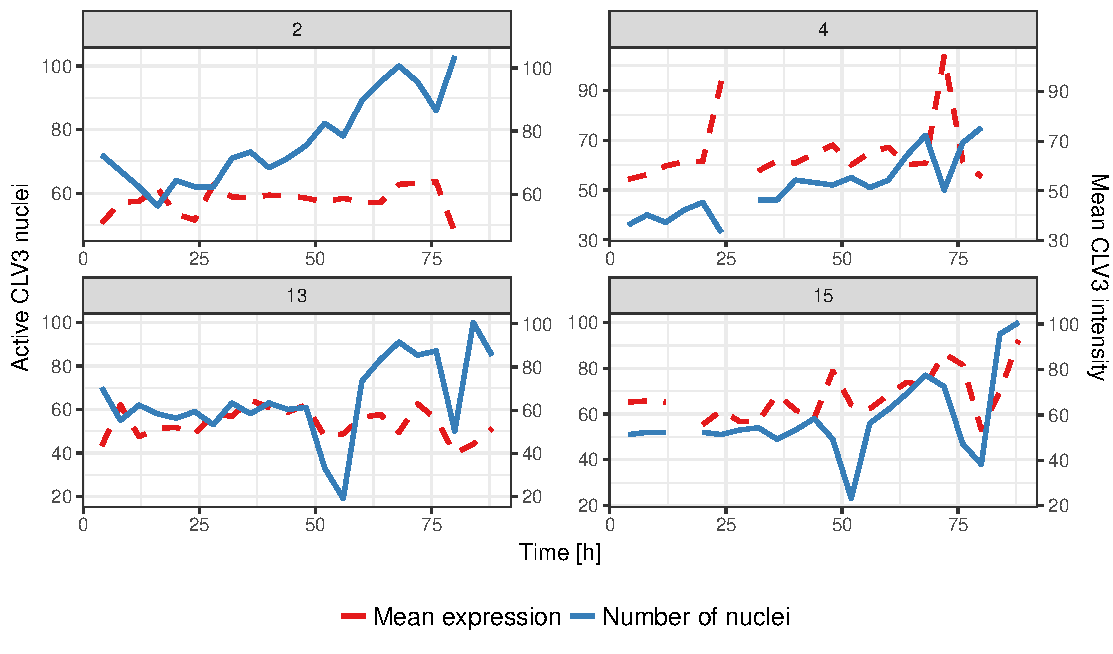
\includegraphics[width=.8\textwidth]{nNucl_trajectories.pdf}
  \caption[Number of CLV3 nuclei over time]{Number of CLV3 nuclei (red)
    over time, as mapped next to the mean nuclear intensity (blue). All plants exhibit
    an increase in the number of nuclei over time, and appear to fluctuate in a
    systematic manner. The mean intensity occasionally shifts in accordance with
    the number of CLV3 nuclei, but in a non-systematic manner.}
  \label{fig:clv3_trajs}
\end{figure}

\begin{figure}[H]
  \centering
  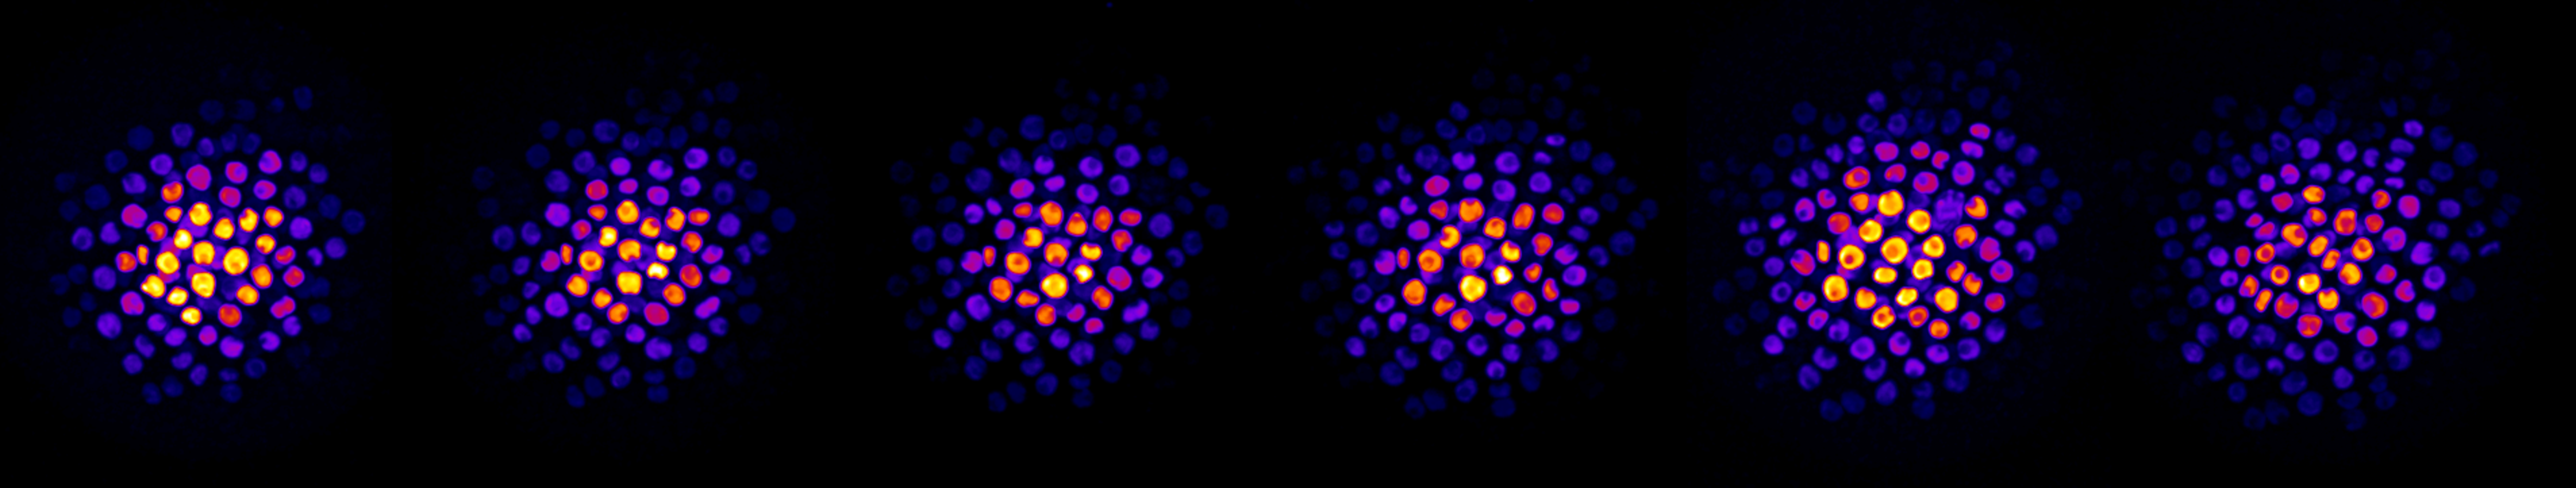
\includegraphics[width=\textwidth]{visual_osc.pdf}
  \caption[Raw image CLV3 domain fluctuations]{Visually observable fluctuations
    in the CLV3 domain. Images are taken from plant 4 in a linear fashion
    between 56 and 76 hours.}
  \label{fig:visual_osc}
\end{figure}

In order to assess the extent of the fluctuations, the lines were detrended using
a second order Loess fit to each curve (\cref{fig:detrended}). When thereafter performing a continuous time
Fourier transform to extract amplified modes, we see that the plants are
biased towards the fourth mode, i.e.\ a period of $\sim$16~hours, in each
respective transformation (\cref{fig:periodogram}).
\vspace{2em}

\begin{minipage}{\textwidth}
  \begin{minipage}[t]{0.47\textwidth}
    \centering
  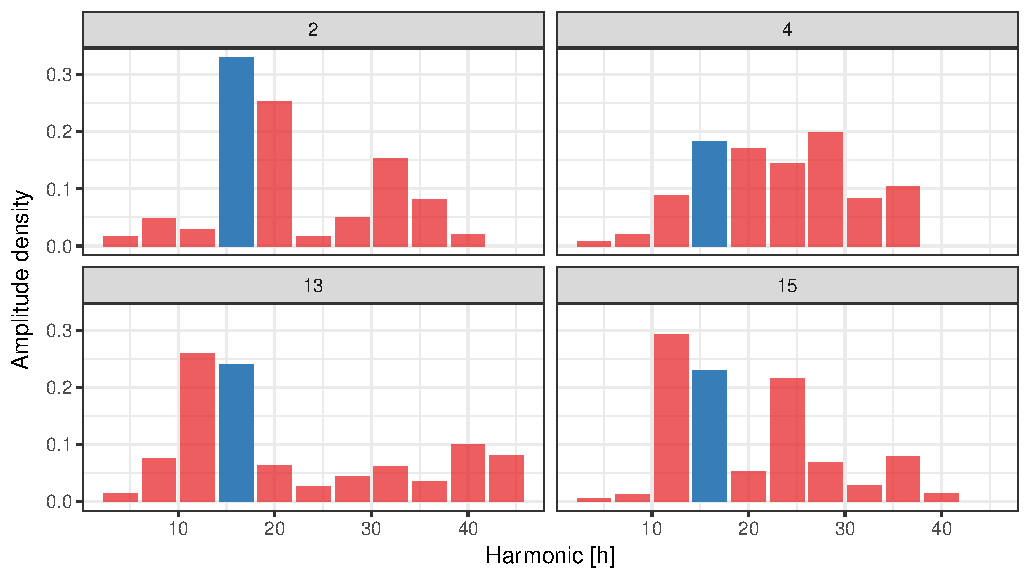
\includegraphics[width=.95\textwidth]{periodogram.pdf}
    \captionof{figure}[Periodogram of nuclear trajectories]{Plant-wise periodogram for detrended number of nuclei
      trajectories. All plants show an emphasised fourth harmonic (blue),
      denoting periodicity with a 16-hour period.}
    \label{fig:periodogram}
  \end{minipage}~~
  \begin{minipage}[t]{.47\textwidth}
    \centering
    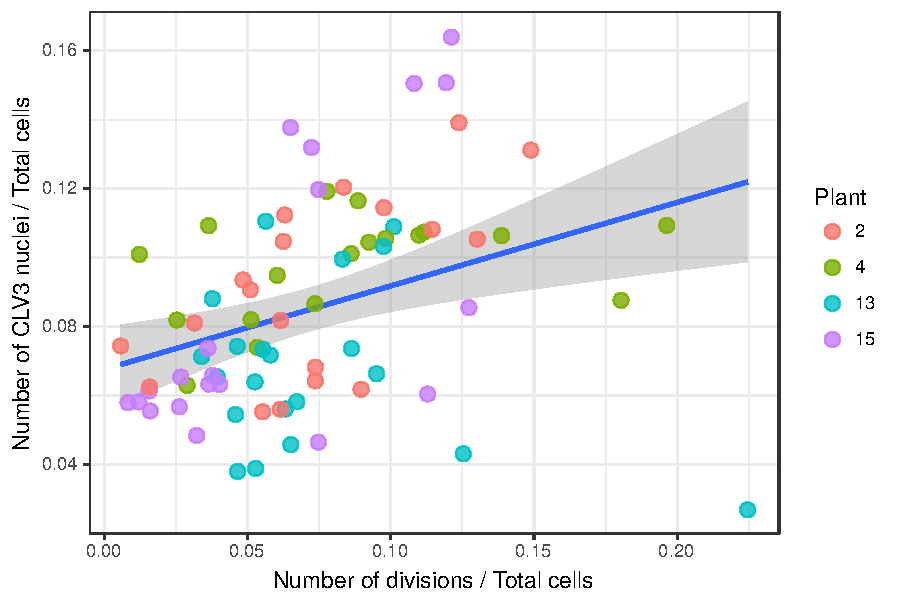
\includegraphics[width=.95\textwidth]{corr_nNucl_nDivs.pdf}
    \captionof{figure}[Link between number of nuclei and number of divisions]{The number of division events correlates linearly
      with the number of CLV3 nuclei, signifying a functional variation due
      to the number of CLV3 nuclei.
    }
  \end{minipage}
\end{minipage}

% and are hence not circadian
\vspace{2em}
In addition to the apparent periodicity, the number of division events
correlates strongly (p = 0.002) with the number of active CLV3 nuclei when normalised by the
total number of cells observed, showing that the number of divisions scales with
the size of the CLV3 domain.


\section{CLV3 expression is stable for apical cells}
Variance in the expression of CLV3 is suppressed in the apical cells
(\cref{fig:clv3d2t}). Generally, the CLV3 distribution assumes a  
shape with low variance close to the apex, larger variance at intermediate
distances, and again low variance at larger distances. 
This appears true for all plants, although plant
13 in particular shows tendencies of having a few weakly expressing apical cells at
several timepoints. It should however be noted that it is possible that errors
in the tracking produces this type of data, and that these outliers vanish when
defining the apex through the weighted expression approach. 

Closer investigations in the distribution of expression
values at distinct distances shows non-bimodal tendencies. Instead, the data
suggests an apparent CLV3 gradient, proportional to the distance to the apex
more in radial terms than in state-wise ones.

\begin{figure}[H]
  \centering
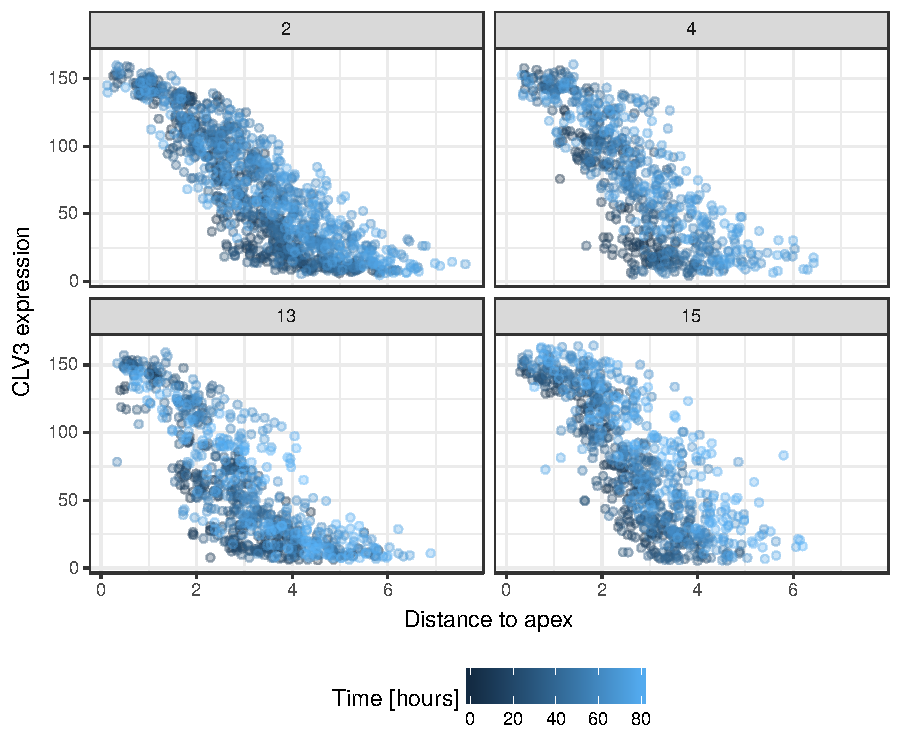
\includegraphics[width=.9\textwidth]{clv3_vs_d2t.pdf}
  \caption[CLV3 distributions]{CLV3 expression distributions for the L1, with the apex of the
    meristem defined as the mean coordinates of the 4 topmost expressing cells
    at each given timepoint. The distributions all assume a hysteresis-like
    appearance, with minor variance at the apex, a highly variable body, and a
    tail with low variance.}
  \label{fig:clv3d2t}
\end{figure}

Using a simple model mimicking the epidermis, it was possible to
replicate the shape of the distribution assuming enzymatic CLV3 activation by a WUS gradient
(\cref{fig:model1}). The enzymatic activation is in this formulation necessary in order to
attain the sigmoidal shape of the curve.




\begin{minipage}{\textwidth}
  \begin{minipage}[t]{0.39\textwidth}
    \centering
    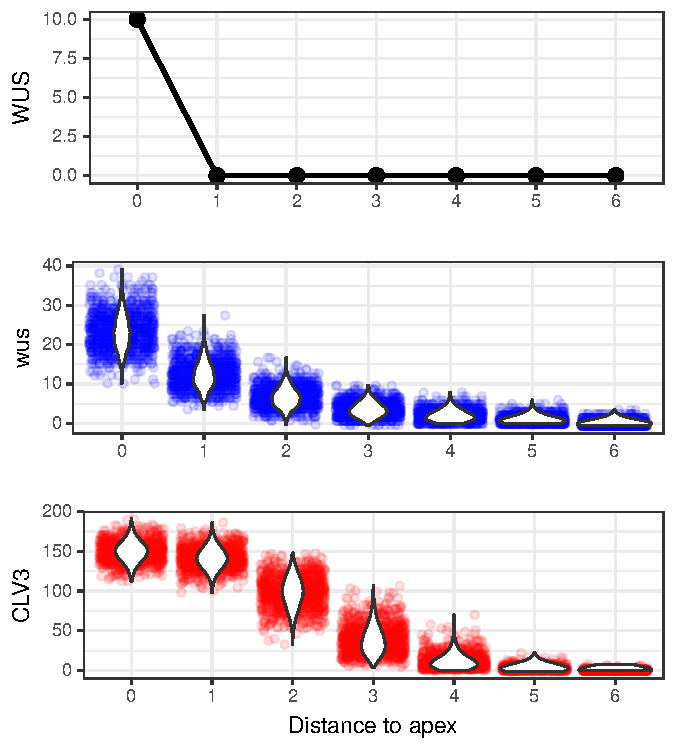
\includegraphics[trim={0 0 0 0cm}, clip, width=.95\textwidth]{model1_results.pdf}
    \captionof{figure}[Epidermis model]{Epidermis model recreating the results
      observed in
      \cref{fig:clv3d2t}. Here, a gradient of WUS induces sufficient
      activating mechanics for producing the correct CLV3 gradient.}
    \label{fig:model1}
  \end{minipage}~~
  \begin{minipage}[t]{.59\textwidth}
    \centering
    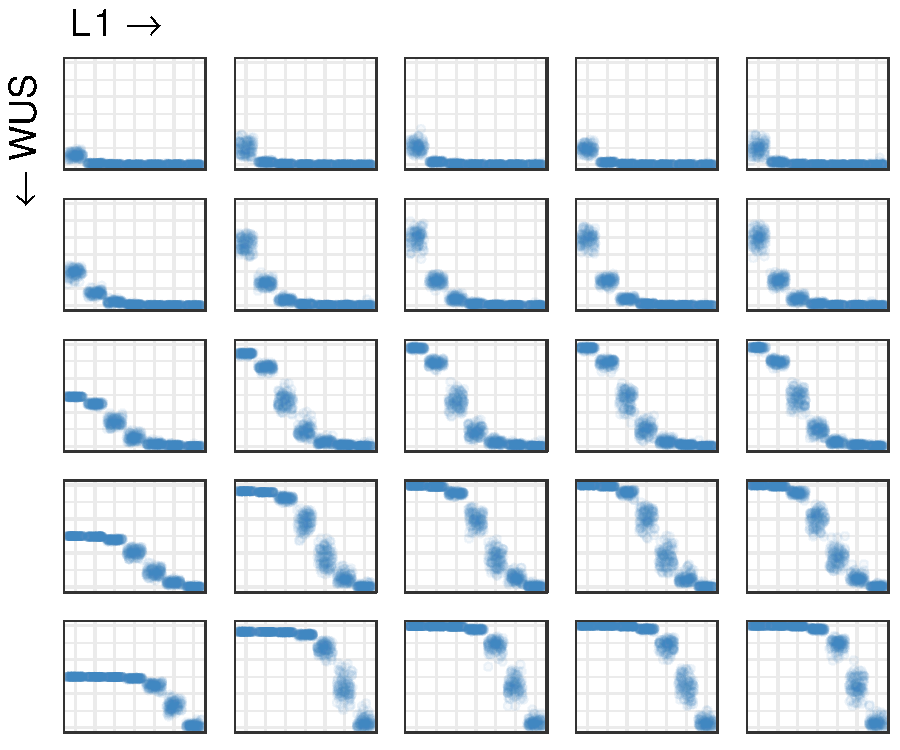
\includegraphics[trim={0 0 0 0cm}, clip, width=.95\textwidth]{l1_wus.pdf}
    \captionof{figure}[L1 model]{Epidermal model recreating the observed
      layer-wise shift in \cref{fig:epireg} (right). Concentrations range from
      2 to 32 concentration units in steps of powers of two. Central regions
      correspond to the observed epidermal case, where the bottom left
      corresponds to the L2 regime, with lower L1 activation, and higher WUS.
      Note that our definition of the apex and the distance to this differs
      slightly from the one in the data.}
    \label{fig:model2}
  \end{minipage}
  \vspace{1cm}
\end{minipage}

Aside of the CLV3 distribution in the L1, we observe a layer-wise separation of
the CLV3 expression in the comparison between
L1 and L2 (\cref{fig:epireg}). In L1, the correlation between
CLV3 expression and nuclear volume appears sigmoidal, although consideration
should be taken to the fluorescence saturation due to the laser. 

In contrast, both L2 and L3 have linear volume-expression relationships,
indicating the possibility of epidermal  
activation, or alternatively subepidermal repression, for creating the differing
distribution shapes. We also see the potential of such a regulatory mechanism in
the distributions of CLV3 expression in relation to the distance to the apex,
where L1 and L2 again behave differently.

The shift in expression between the L1
and L2 with respect to the  
distance to the apex is captured conceptually by our second model
(\cref{fig:model2}), where the
epidermal state is in the central regions, with high L1 signal, and intermediate
WUS. The L2 state could correspond to the leftmost bottom end of the facet, with
higher or equivalent WUS signal, and lesser L1 activation. One could also
imagine e.g.\ L1-signal induced mutants, which in our model would be shifted to
the right in the facet.

\begin{figure}[H]
  \centering
  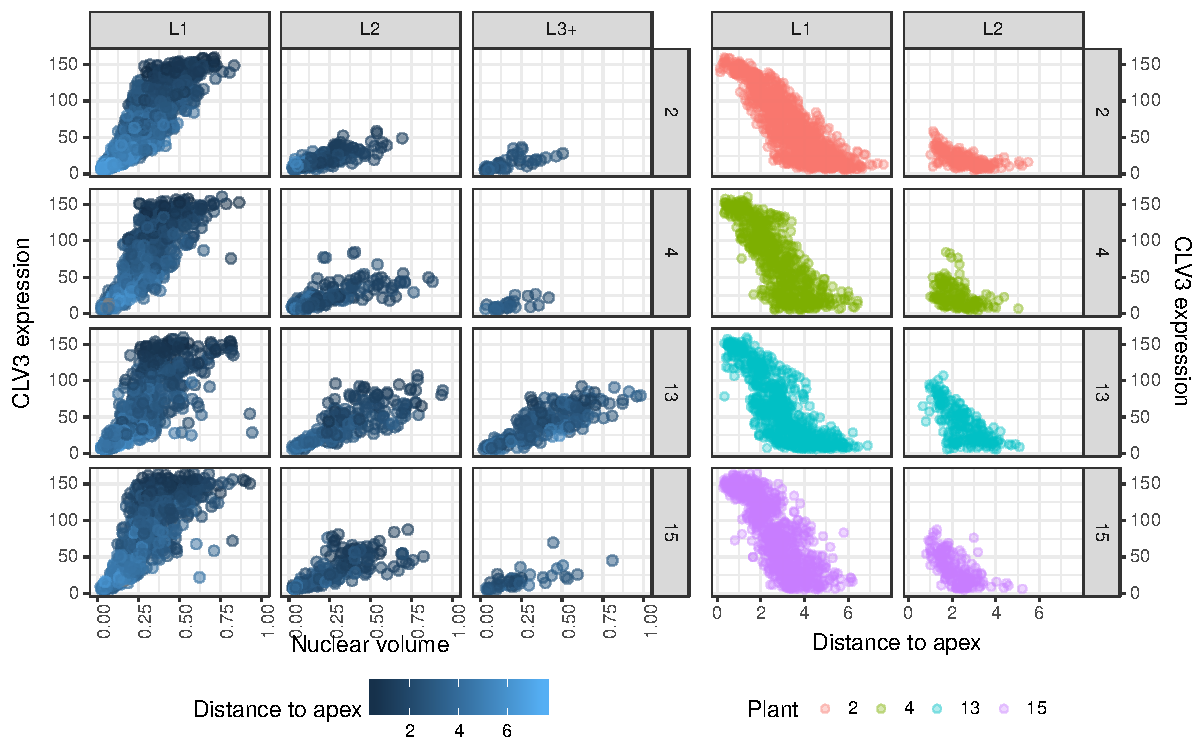
\includegraphics[width=\textwidth]{epireg.pdf}
  \caption[Cues of epidermal regulation]{Distribution data suggest differing
    regulation between L1 and the subepidermal layers. In penetrating deeper
    into the tissue, the CLV3 expression relative the nuclear volume changes
    from a sigmoidal to linear relationship (left). Similarly, the CLV3
    expression relative the distance to the apex appears to have similar shape
    in the L2 as in the L1,
    but shifted.}
  \label{fig:epireg}
\end{figure}

%\section{Distribution shifting suggests epidermal regulation}
%\subsection{CLV3 is induced in the epidermis}

 % This holds regardless of what distribution looks like

 \section{Functional clustering implies slow dsRED degradation}
 The apical cells appear to be clustered functionally, suggesting that a
 significant portion of the CLV3 expression observed outside of these topmost
 cells may in fact be reporter remnants, stemming from the decay time of the
 dsRED reporter. 
 
 \Cref{fig:mvol_apex} shows a tendency of the apical cells to
 assume a differing average membrane volume between cells at the apex (distance
 0), and the
 ones neighbouring (p = 5e-12, 1e-2, 7e-4, 7e-5). This
 contrasts with the observed nuclear volume, where instead an overall decreasing
 trend in the response to CLV3 appears (\cref{fig:nvol_apex}).
 
 In addition, the topmost cells undergo significantly fewer divisions per cell in
 that region as opposed to the other cells in the L1 (\cref{fig:nDivs_apex}).
 Most division events instead appear to be focused in the first to third cell
 layer away from the apex, and thereafter decline. Under the assumption that the
 number of cells scale with the area such that $N \propto r^2$, we should expect
 to see the number of division events increase linearly with $r$; here we
 instead see the linear tendency only for cell distances 1-3, where the topmost cells
 behave differently. Generally, the observations can be observed in three
 points:
 \begin{enumerate}
   \item Topmost cells divide less frequently than cells in layer 1-3
   \item Cells in layers 1-3 divide at a similar frequency per cell
   \item At cell distances $>3$, the number of divisions per cell decreases
     steadily
 \end{enumerate}

 % Discussion: Growth rate
 % Discussion: Fuzziness due to definition

 \begin{figure}[H]
   \centering
   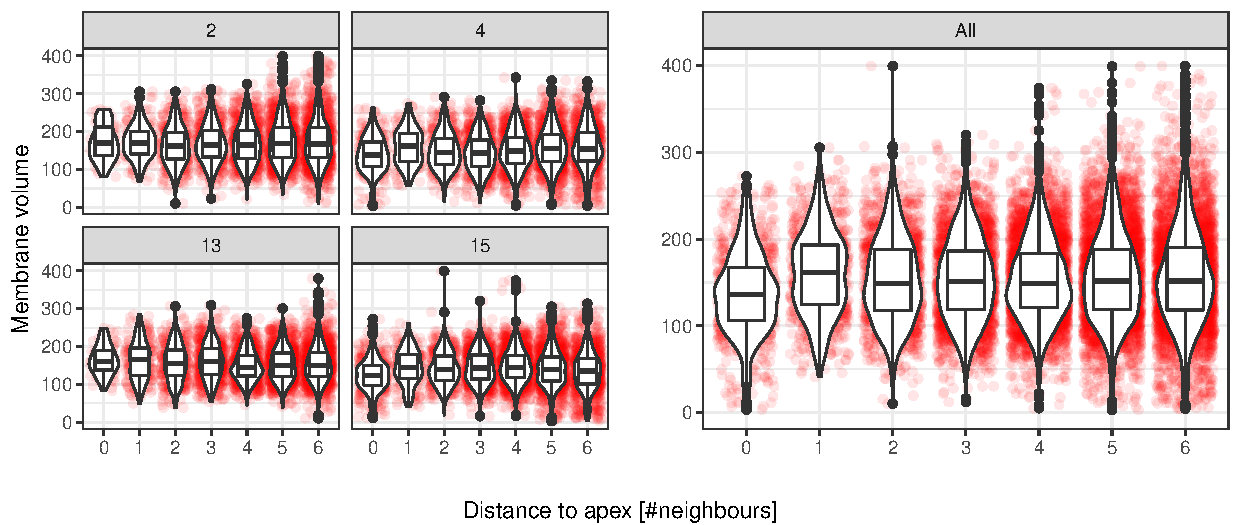
\includegraphics[width=\textwidth]{mvol_apex.pdf}
   \caption[Membrane volume clustering]{Membrane volumes in the L1 clustered at different distances from the apex in
     number of cells. Cells as part of the apex here are defined as the 4
     topmost expressing cells; their neighbours in turn correspond to the cells
     at distance 1, and so on. Here all examples but plant 2 have a
     statistically significant separation of average membrane sizes between
     distance
     0 and  1. Note also the maintained average volume at farther distances, in
     contrast to \cref{fig:nvol_apex}.}
  \label{fig:mvol_apex}
\end{figure}

\begin{figure}[H]
   \centering
   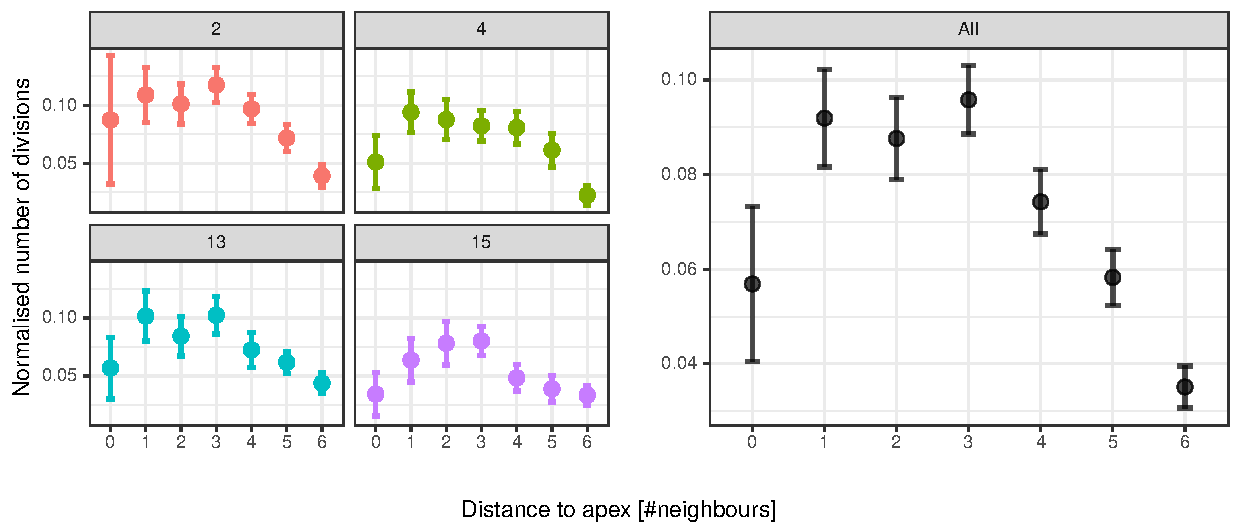
\includegraphics[width=\textwidth]{nDivs_apex.pdf}
   \caption[Division rate clustering]{Division analogue to \cref{fig:mvol_apex}, with the average number of
     divisions normalised by the number of cells at that corresponding
     distance, along with the standard error of the mean. As in the membrane
     volume case, plant 2 shows a different trend  
     than the other plants and in particular exhibits a larger variance,
     showing noise in the definition of the topmost cells. 
   }  
   \label{fig:nDivs_apex}
\end{figure}

Separating out the lineages which are present throughout the full time course
reveals an apparent contained maintenance of roughly four cells where decline in the
CLV3 expression can not be noted (\cref{fig:trajectories}; lineages 7, 16,
17). Overall, cells appear to be in either one of two state with respect to
the rate of change of their CLV3 expression, in a few select trajectories, where
further analysis indicates that cells  
assume a declining state when pushed out of the very apex. Cells that in
contrast remain in this region maintain their high expression profiles,
signifying the possibility of only the very apical cells effectively expressing
CLV3. 

It is unclear whether the resolution of the trajectories is significant
enough to observe the exponential decay in dsRED, or whether a linear
approximation is sufficient. \Cref{fig:dsred_decay} shows these two alternatives
where the interpretation of the half-life differs with a factor of two depending
on the interpretation, where the exponential one corresponds to a half-life of
roughly 41.7 hours, and the linear correspondingly 83.3 hours, assuming a Taylor
expansion to the first order. 

\begin{figure}[H]
  \centering
  \begin{minipage}{\textwidth}
    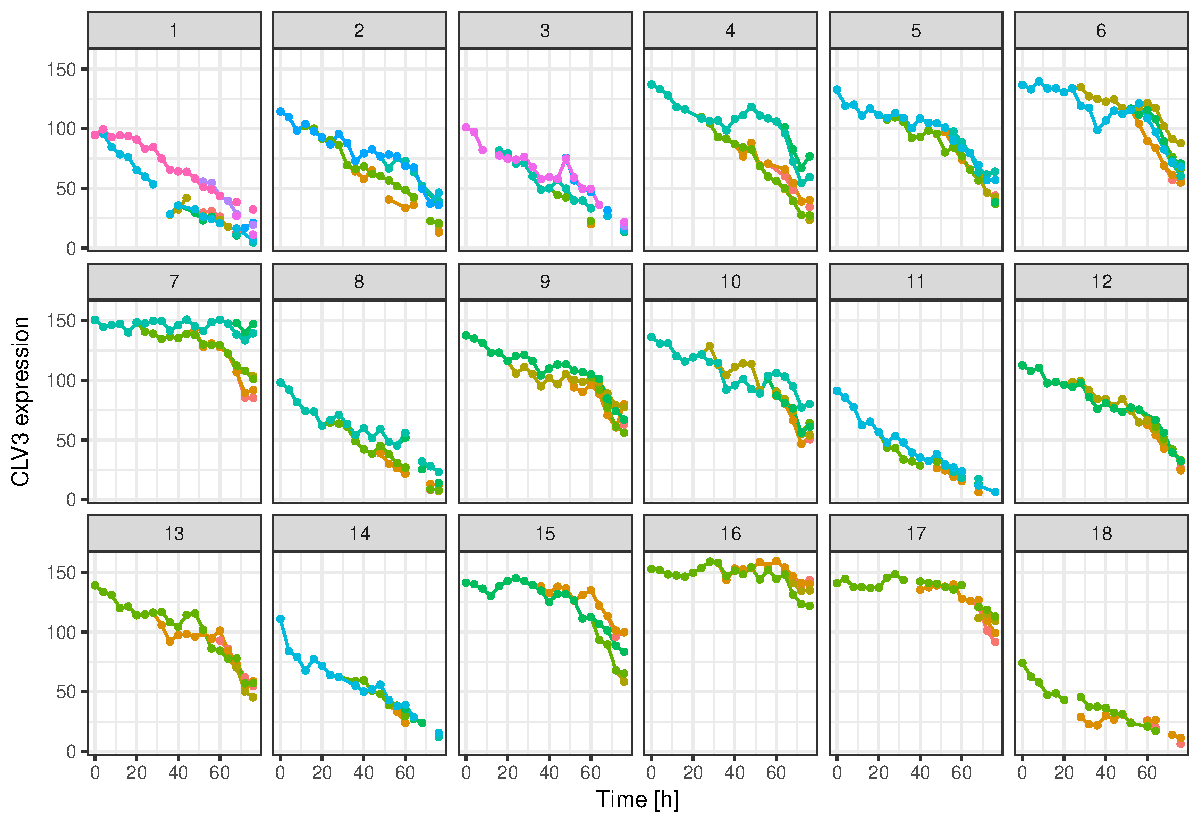
\includegraphics[width=\textwidth]{plant2_trajectories.pdf}
    \vspace{1cm}
      \centering
      \begin{minipage}{0.39\textwidth}
      \centering
      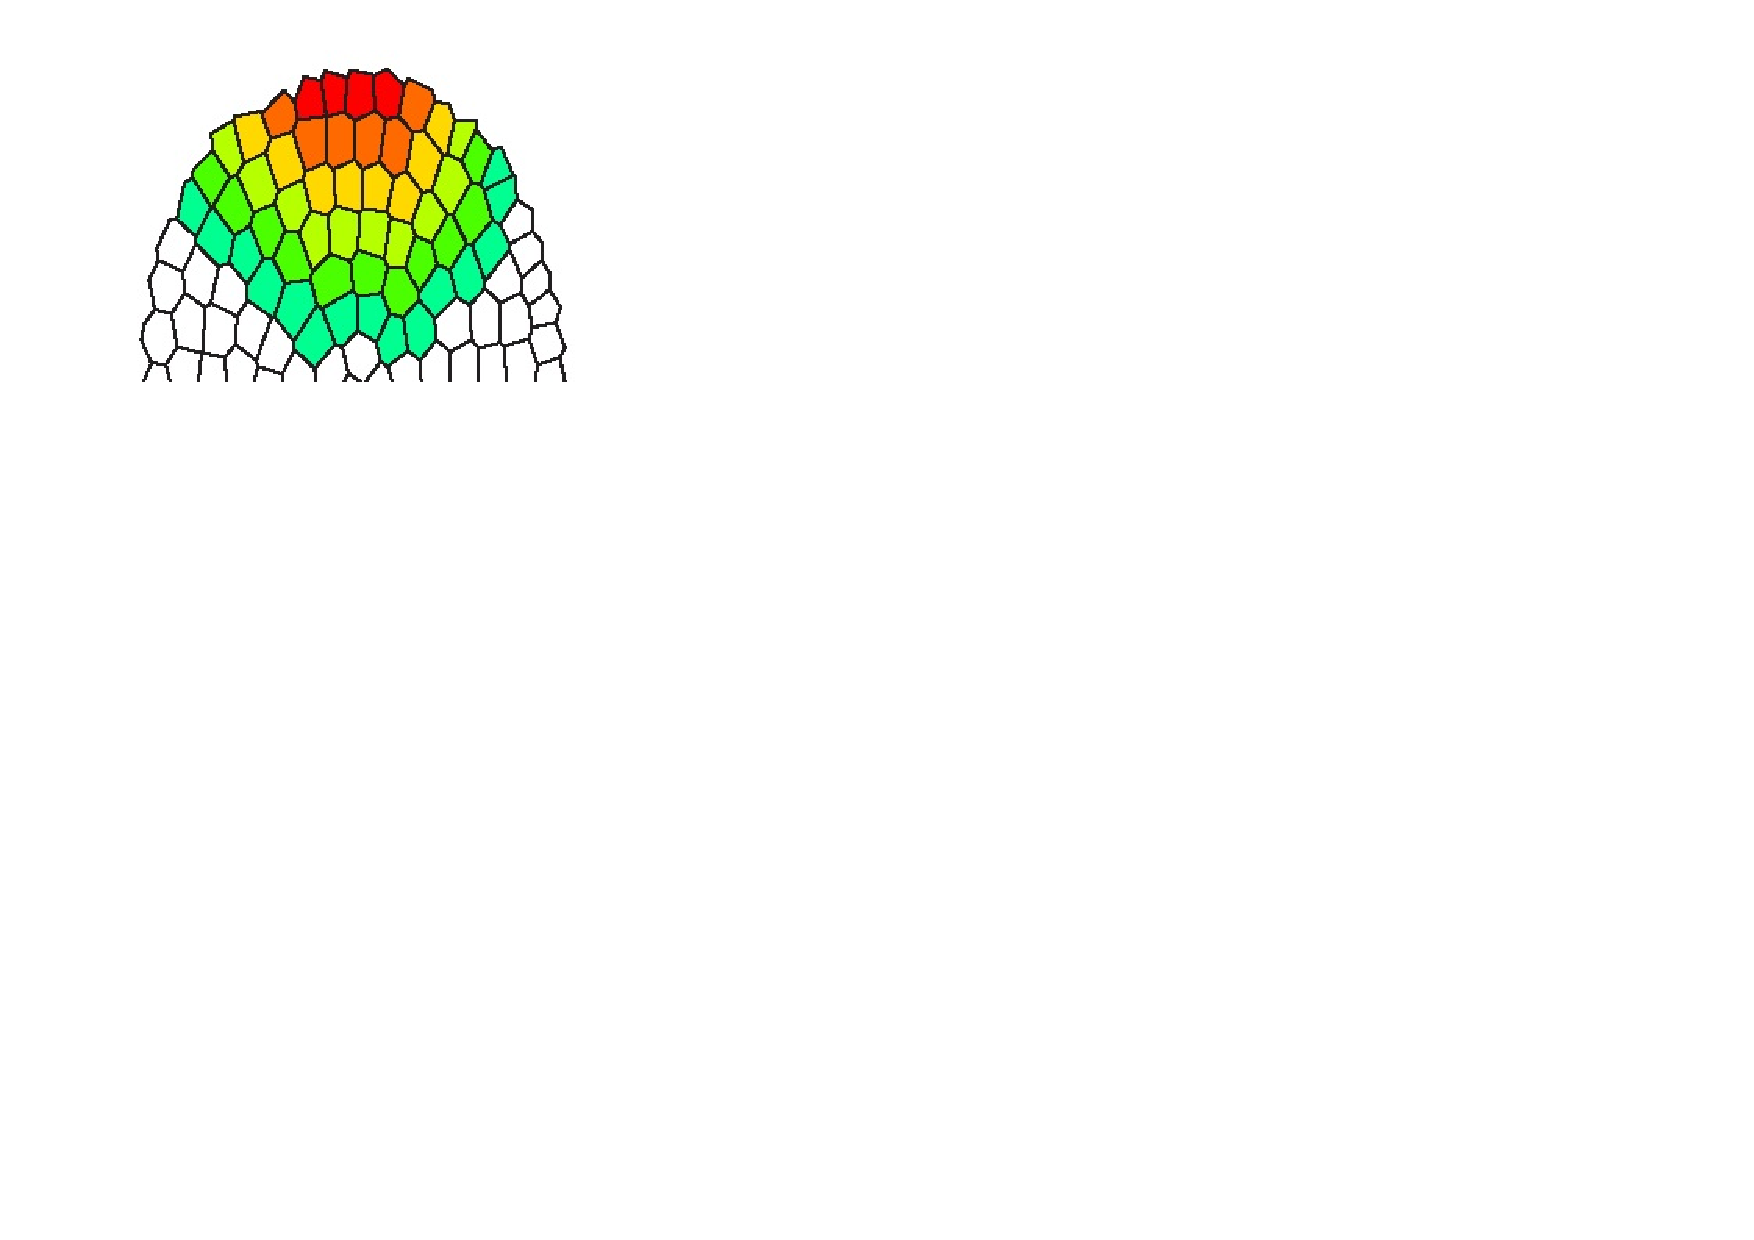
\includegraphics[trim={2cm 15.3cm 20cm 0}, clip, width=.95\textwidth]{apex_definition.pdf}
    \end{minipage}\hfill
    \begin{minipage}{.59\textwidth}
      \centering
      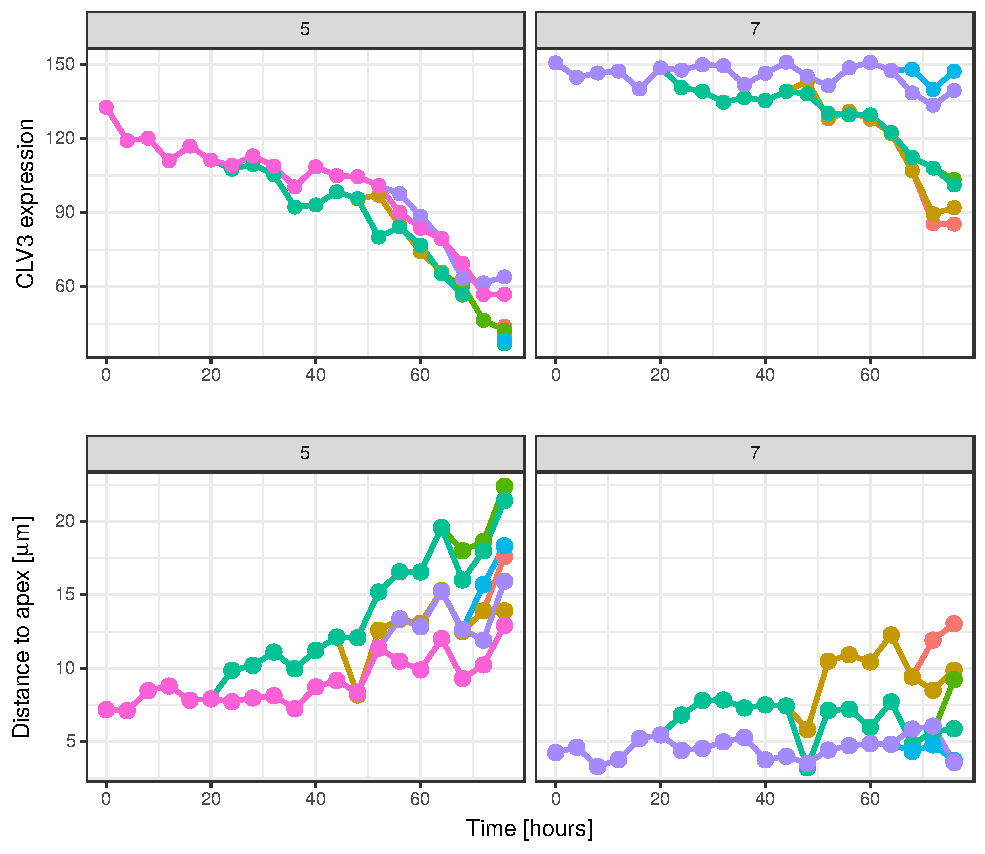
\includegraphics[width=.95\textwidth]{select_trajectories.pdf} 
    \end{minipage}
  \end{minipage}
  \caption[Cell line trajectories]{Cell line trajectories for lineages in plant 2 with cells present
      at both the initial and final timepoint in the series. Cells generally
      have a declining or maintained behaviour corresponding to the two cases
      (cell line 5 and 7)
      emphasised in the bottom right. This corresponds to the behaviour
      illustrated in the bottom left, with cell lineages at the very top having
      preserved expression levels (red), and decreasing signal outside outside of
      this region. Missing timepoints in trajectories in most cases correspond
      to data filtered out due to division events (see \cref{sec:filtering}).}
    \label{fig:trajectories}
\end{figure}

\begin{figure}[H]
  \centering
  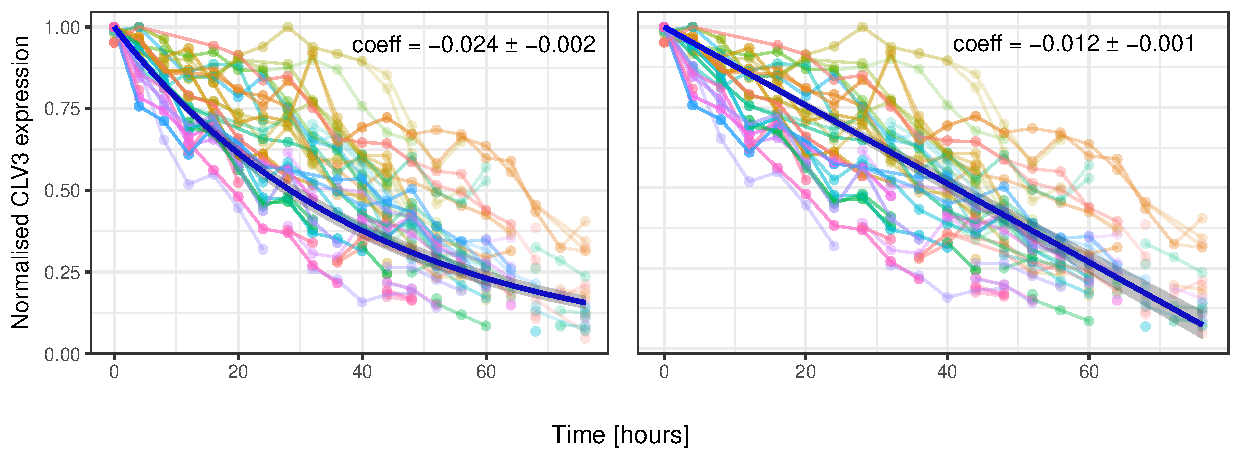
\includegraphics[width=\textwidth]{dsred_plant2.pdf}
  \caption[Approximation of dsRED decay]{Exponential and linear approximation of
    dsRED decay respectively. Data shows plant 2, with all sublines with at
    least 12 data points, down-shifted to timepoint 0 hours for comparison, and
    divided by the timeseries maximum.

    Fitted lines are taken as the mean coefficients of singular fits to each
    individual line, presented with the 95~\% confidence interval.
    Also plants 4, 13 and 15 produce results within the margin of errors for
    both approximations.
  }
  \label{fig:dsred_decay}
\end{figure}

Assuming a situation where dsRED is not produced, we can make a first
approximation of the expected rate CLV3 decays as a function of distance to the apex. Given
that cells are on average pushed out of the CZ at a rate $\dot R = k_R$, the
rate of change for the CLV3 expression can be written on the form 
\begin{align*}
  \dot C = \frac{\dd C}{\dd t} &= \frac{\dd C}{\dd R} \frac{\dd R}{\dd t}
  \Rightarrow \\
  \frac{\dd C}{\dd R} &= \frac{1}{k_R} \frac{\dd C}{\dd t} 
  \label{eq:decayrate}
\end{align*}
where $R$ denotes the radial distance. Under exponential CLV3 decay, e.g.\ $\dot C =
-k_{C}C$, CLV3 should decay with the radius as $\frac{\dd C}{\dd R} =
\frac{k_{C}}{k_{R}}$, which appears possible given the distribution in
\cref{fig:clv3d2t}. Note that this primarily serves as a first approximation,
and that it in longer timescales should be appropriate to consider also
exponential growth.

\section{Long-lived cells tend to amass centrally in the deep tissue}
When investigating number of hours for which a cell is observed before having
divided, we attain an apparent bimodal distribution of division ages which
is pronounced in the deeper tissue (\cref{fig:age}). In particular, a set of cells
are clustered at an age corresponding to roughly  
$3\times$ the normal cell cycle in the deeper layers. Notably, this effect is
not accompanied by a similar cluster at $2\times$ the normal cell cycle length, which
would be expected in the event of missed divisions in the tracking. The effect
is especially noticeable in plants 2, 4, and 15 (\cref{fig:age_all}), where all
of these show an amassment of division events at the 60 hour mark, most
protruding in the L3.   

\begin{figure}[H]
  \centering
  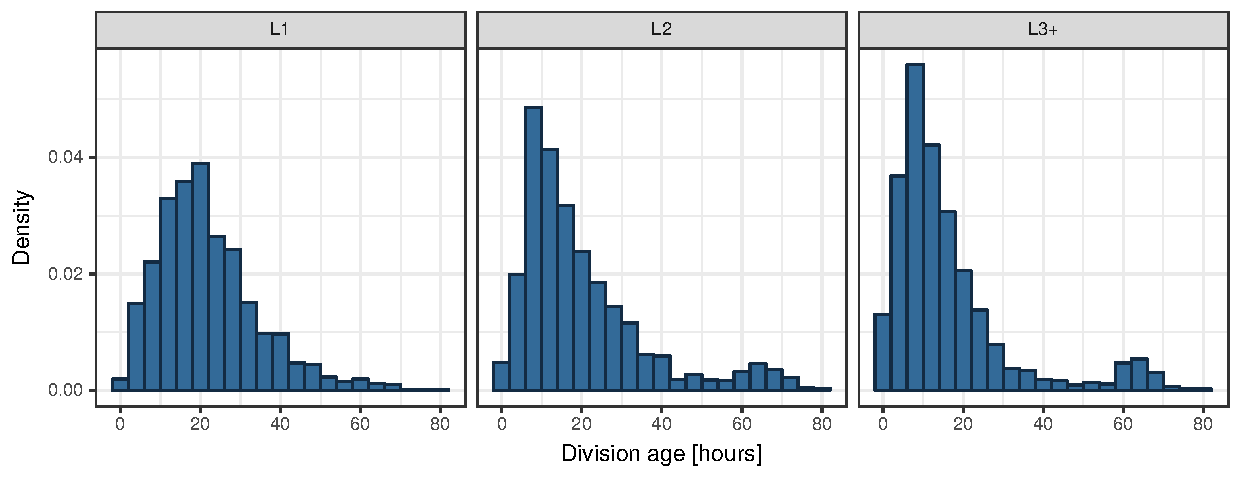
\includegraphics[width=\textwidth]{age.pdf}
  \caption[Layer-wise age distribution]{Distribution of ages before division. The subepidermal layers have an
    amassment of cells dividing around the 60 hour mark, i.e.\ at ca 3$\times$
    the normal cell cycle.}
  \label{fig:age}
\end{figure}

\begin{figure}[H]
  \centering
  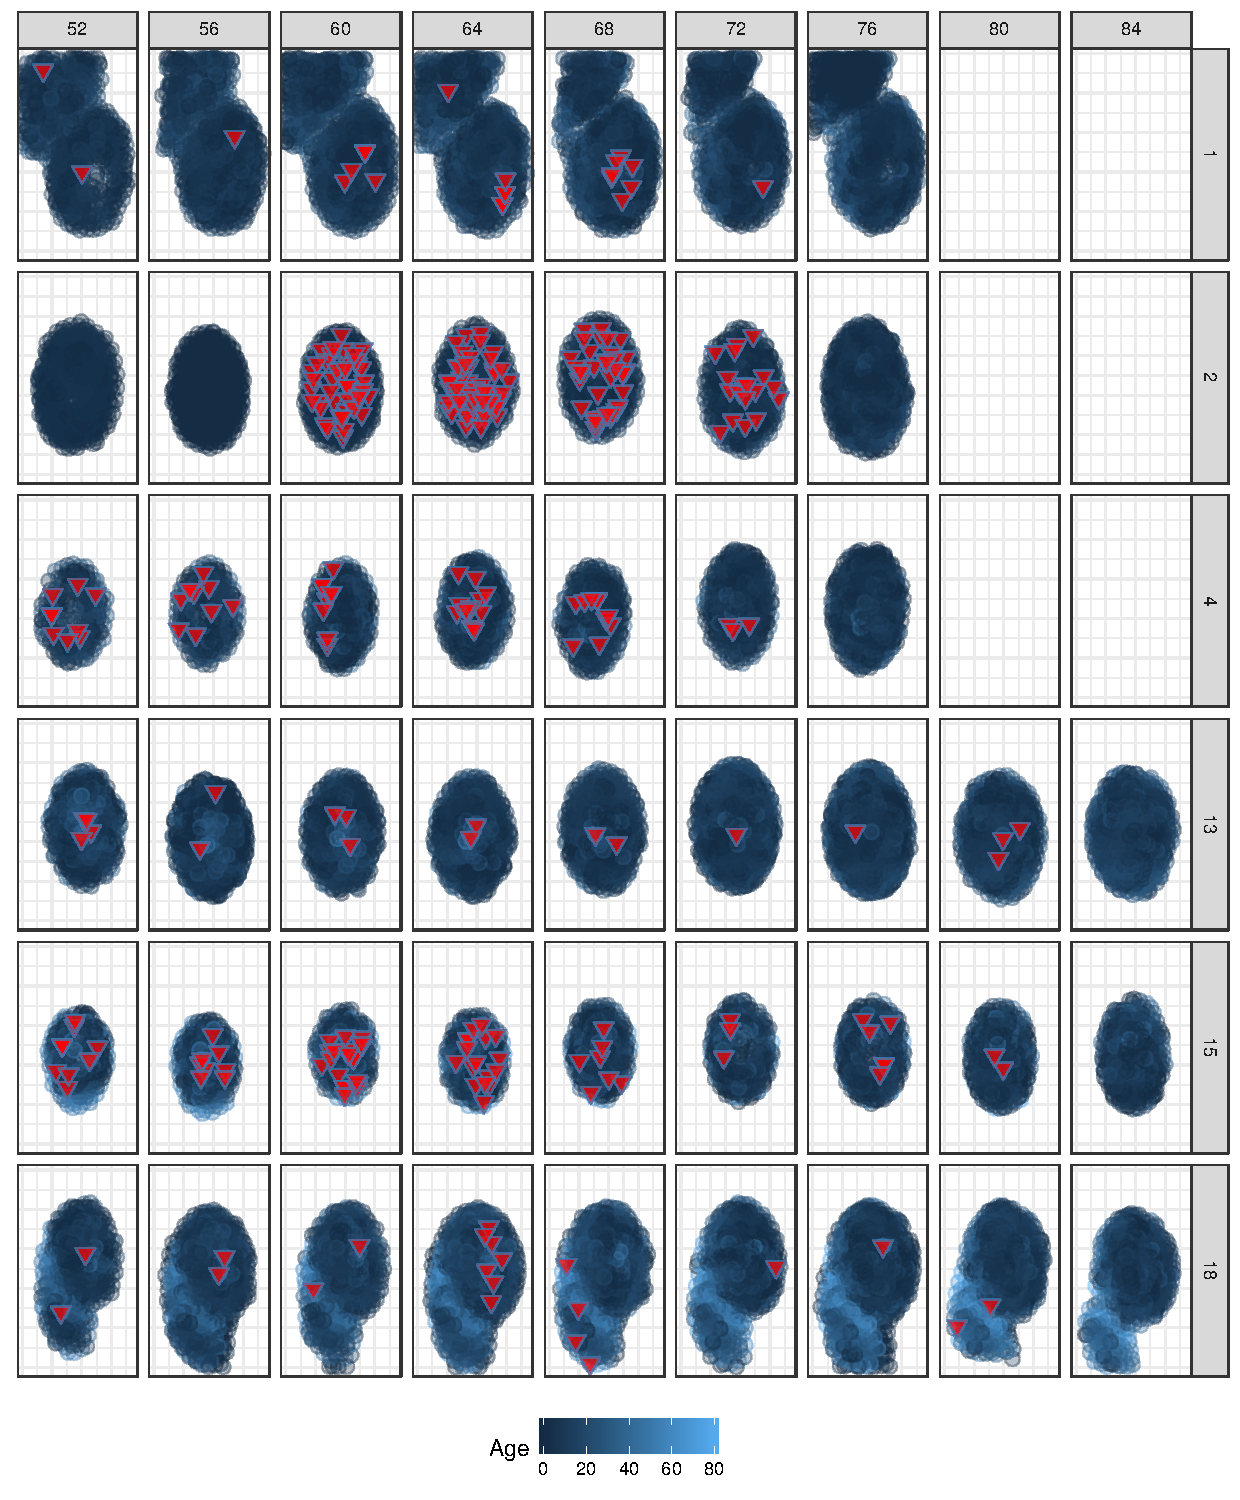
\includegraphics[width=\textwidth]{ages_52plus.pdf}
  \caption[Clustering of high-longevity cells]{Cell coordinates grouped by plant and time for cells not in L1, coloured by age, with division events for cells with
    age $>48$ denoted as red triangles. There appears to be clustering in the
    center of the meristem in several cases. Note also how primordia are appearing in plants 1
    and 18, and how cells in the boundary between primordia tend to be
    affiliated with higher ages.}
  \label{fig:ages}
\end{figure}

\section{The CLV3 apex does not coincide with the geometric}

\begin{figure}[H]
  \centering
  \begin{minipage}{.8\textwidth}
		\begin{minipage}[t]{0.49\textwidth}
      \centering
			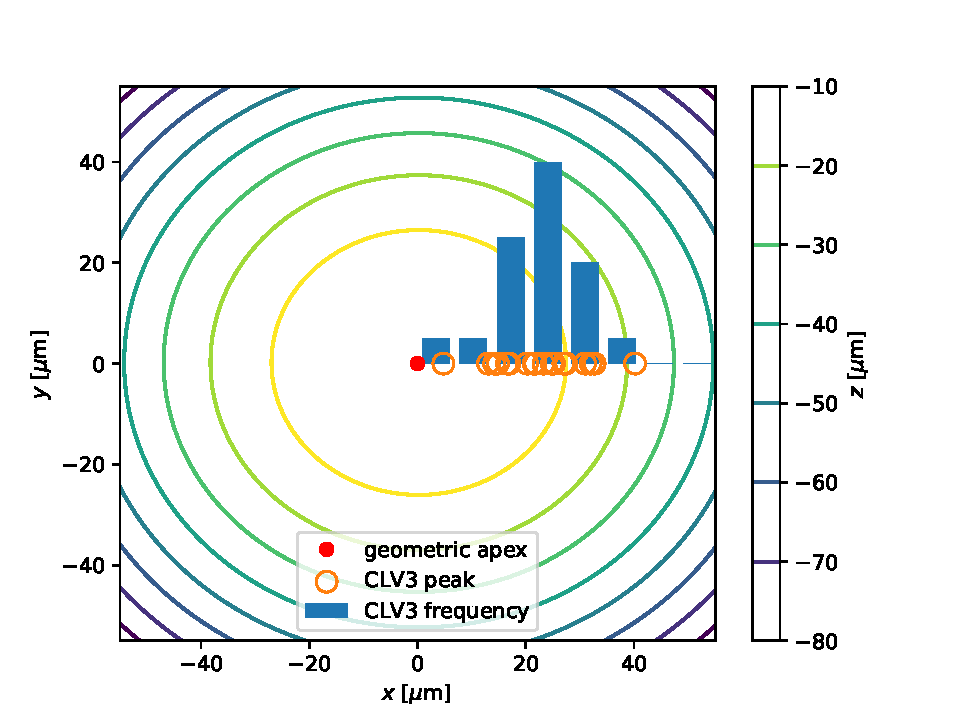
\includegraphics[trim={2cm 1.2cm 4.1cm 0cm},clip,width=.80\textwidth]{plant02.pdf} 
    \end{minipage}\hfill
		\begin{minipage}[t]{.49\textwidth}
      \centering
			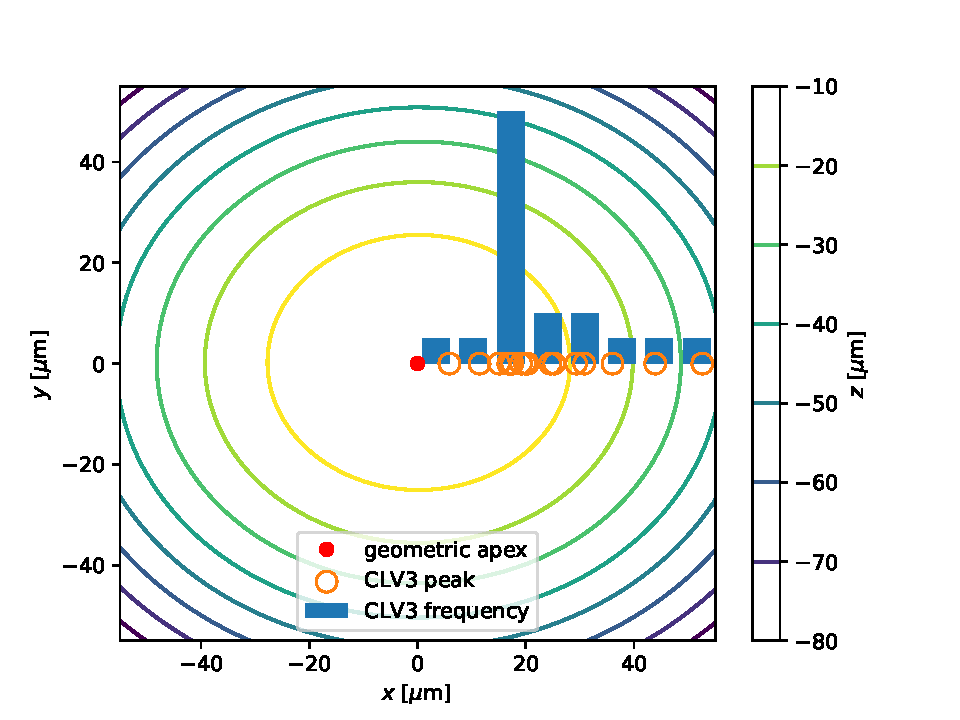
\includegraphics[trim={2cm 1.2cm 1.5cm 0cm},clip, width=\textwidth]{plant04.pdf} 
    \end{minipage}
  \end{minipage}\\
  \begin{minipage}{.8\textwidth}
		\begin{minipage}[t]{0.49\textwidth}
      \centering
			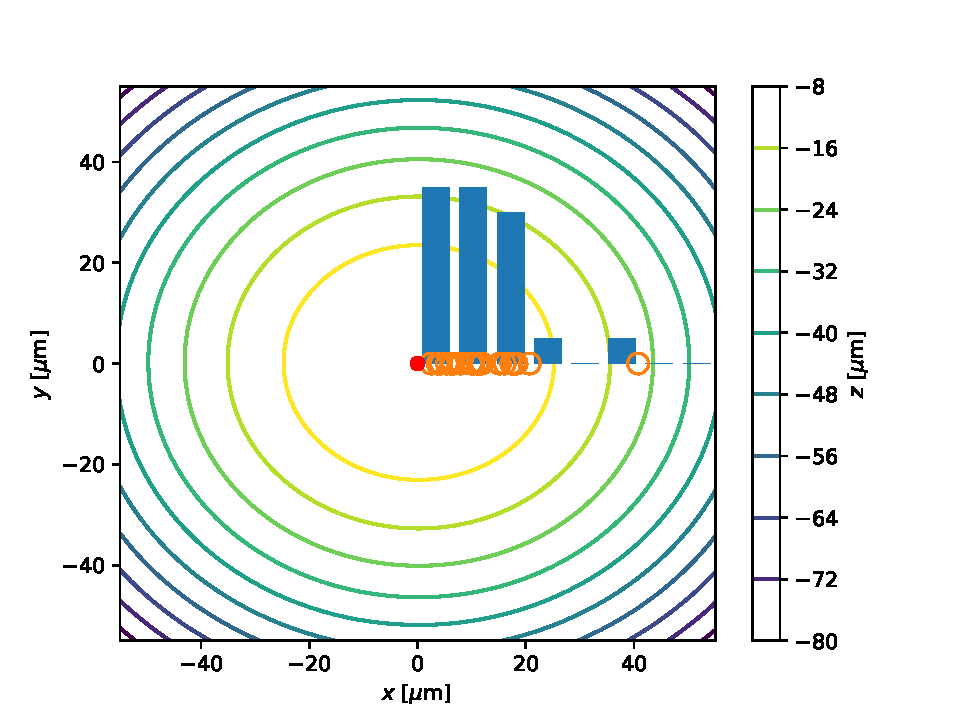
\includegraphics[trim={2cm 0cm 4.1cm 0cm},clip, width=.80\textwidth]{plant13.pdf} 
    \end{minipage}\hfill
		\begin{minipage}[t]{.49\textwidth}
      \centering
			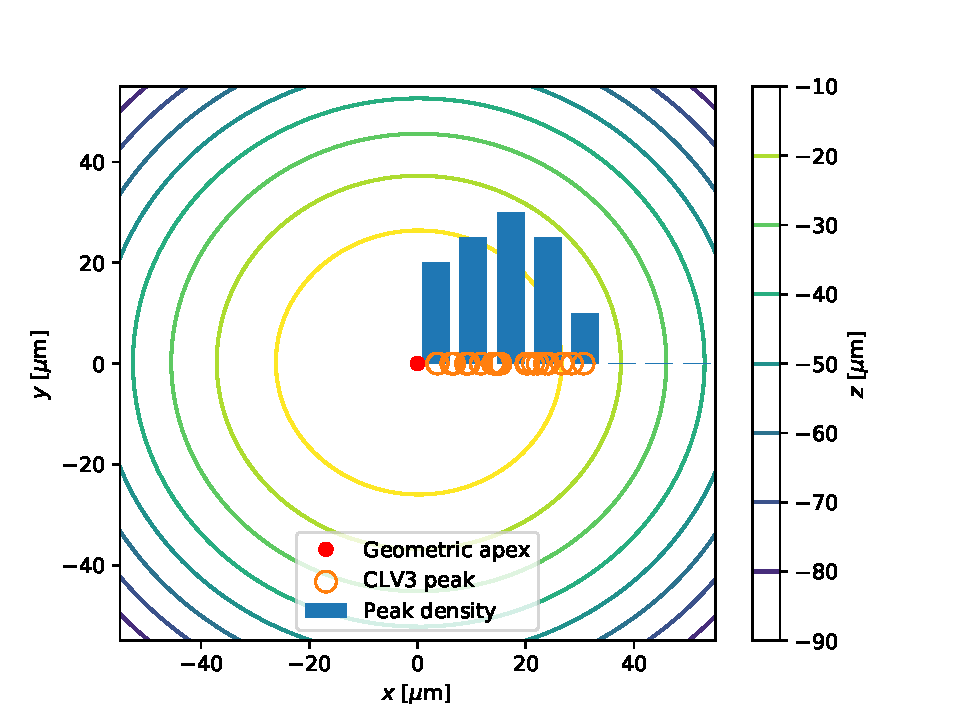
\includegraphics[trim={2cm 0cm 1.5cm 0cm},clip, width=\textwidth]{plant15.pdf} 
    \end{minipage}
  \end{minipage}
	\caption[Comparison between geometric and genetic apex]{Distributions of
    radial distances from the geometric apex, as fitted with a paraboloid shape,
    for plants 2, 4, 13 and 15.
    CLV3 apices are defined as the mean coordinates of the four highest
    expressing CLV3 cells. Notably, all plants have distributions peaking at
    a distance of roughly 10-20 $\mu$m.
  }
  \label{fig:age_clusters}
\end{figure}
Notably, the CLV3 peak and the geometric apex do typically not coincide, with
the CLV3-based apex typically at a distance of $10-20\mu$m, corresponding to 2-4
cells in distance. This is also visually inferrable from the raw channel images
(\cref{fig:apex_center}), where the CLV3 domain can be seen as shifted away from
the structural center.

While the quality of the fit can be affected by the presence
of primordia, the evolution of paraboloid parameters over time is relatively
constant (\cref{fig:para_time}).

\begin{figure}[H]
  \centering
  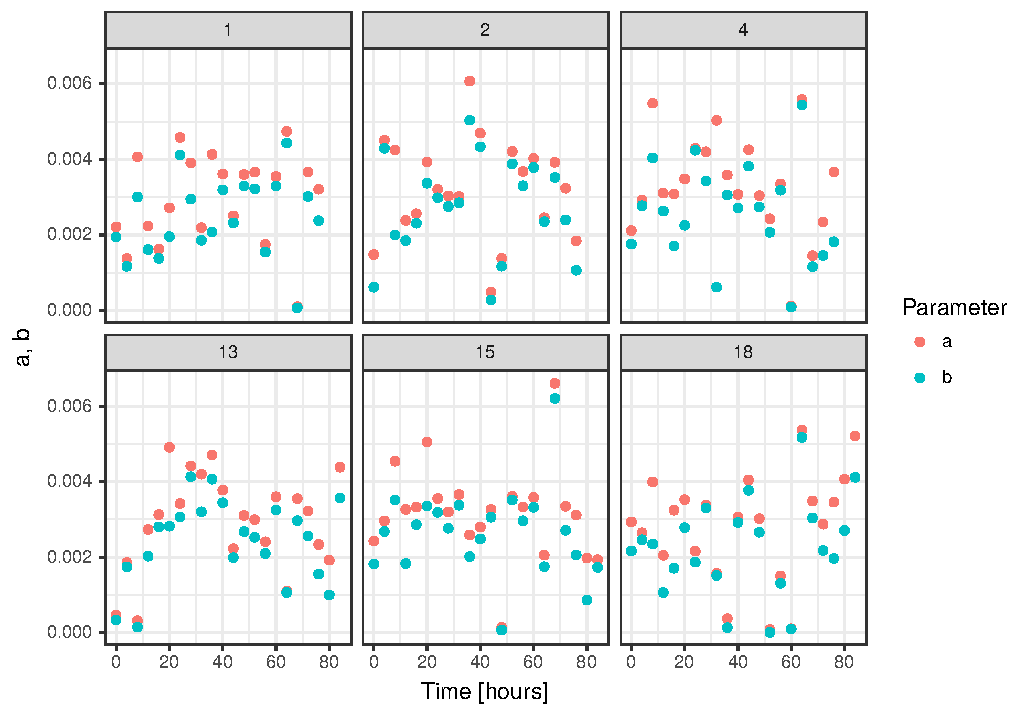
\includegraphics[width=\textwidth]{para_time.pdf}
  \caption[Paraboloid time evolution]{Evolution of paraboloid parameters, where
    the paraboloid has been fit according to the equation $ax^2 + by^2 = z$. We
    have here defined $b$ as determining the axis of largest curvature.}
  \label{fig:para_time}
\end{figure}

For emphasis, we have included an example of the evolution of the largest axis
of curvature for plant 15 (\cref{fig:timeevol_ex}). In general, the paraboloid
shape is on the same order of magnitude between timepoints, demonstrating the reliability in
the definition of the geometric apex. While there are some variations in the
overall curvature, these are generally consequences of the image stack-depth,
and typically only affect the precision of the $z$ coordinate. Since our
analysis is based on a projection to the $xy$ plane, this does not
significantly affect our results.


\begin{figure}[H]
  \centering
  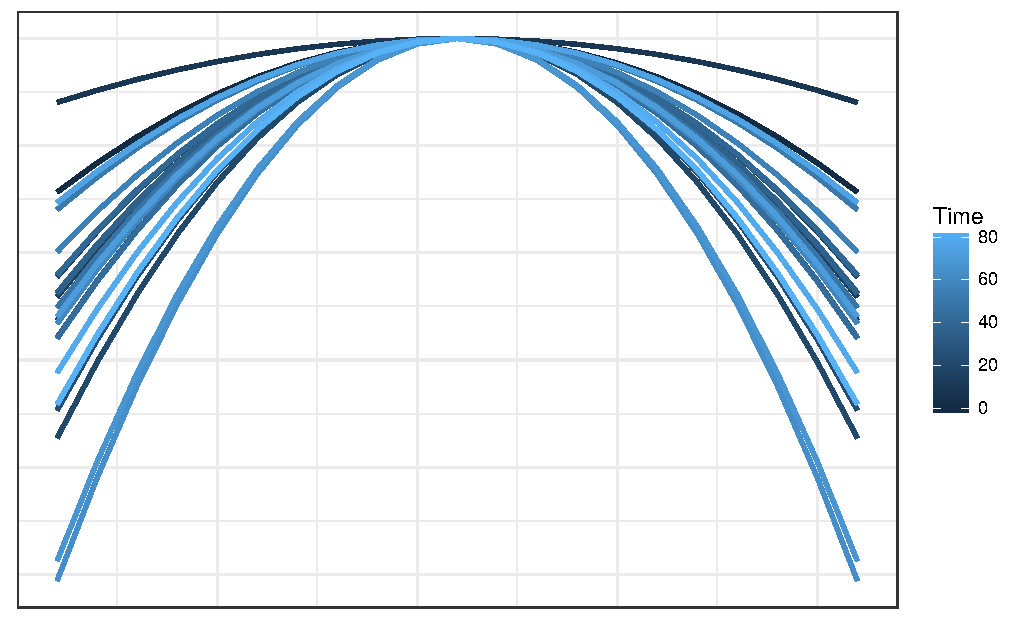
\includegraphics[width=.6\textwidth]{timevol_paravl_15.pdf}
  \caption[Example of paraboloid shape evolution]{Example depiction of evolution
    of paraboloid parameters, taken from plant 15, where
    we have here visualised the axes of curvature according to the equation
    $y = -bx^2$, where $b$ thus has the same significance as in
    \cref{fig:para_time}. One significant outlier can be seen, corresponding to
    $t = 48$ hours; other parabola have curvatures similar in magnitude.}
  \label{fig:timeevol_ex}
\end{figure}
